\documentclass{article}

\usepackage{siunitx} 
     \usepackage[final]{neurips_2019}


\usepackage[utf8]{inputenc} % allow utf-8 input
\usepackage[T1]{fontenc}    % use 8-bit T1 fonts
\usepackage{hyperref}       % hyperlinks
\usepackage{url}            % simple URL typesetting
\usepackage{booktabs}       % professional-quality tables
\usepackage{amsfonts}       % blackboard math symbols
\usepackage{nicefrac}       % compact symbols for 1/2, etc.
\usepackage{microtype}      % microtypography
\usepackage{graphicx}
\usepackage[title]{appendix}

\title{Classification of Mushrooms: Edible or Poisonous}

\author{
Wun-Syuan Wu, Charlie Yang, Ming Zhao 
    \\
    \\
  University of California, Davis}

\begin{document}

\maketitle

\section{Introduction}
\subsection{Motivation}

Driven by the organic food and back-to-nature movements, the popularity of wild mushroom hunting has increased dramatically\cite{Eren2010}, resulting in a substantial rise in mushroom poisoning incidents, with over 7000 incidents have been reported annually in the United States since 1999\cite{Brandenburg2018}. Among the approximately 100,000 known fungi species worldwide, around 100 are toxic to humans\cite{Graeme2014}, and this number is steadily growing with 600 new fungi species discovered each year\cite{Lima2012}.

Contrary to traditional beliefs, toxic mushrooms are not necessarily colorful. Many appear quite ordinary, making visual toxicity inference challenging. Despite these difficulties, the wealth of images of wild mushrooms available offers a unique opportunity. By leveraging these images and domain expertise, we can use computer vision to train machine learning models. This approach offers a potential solution to the challenges inherent in mushroom toxicity identification, creating valuable tools for mushroom enthusiasts and field scientists.

\subsection{Problem Definition}

The main objective of this project includes two parts. It aims to:

\textbf{\emph{(i) Develop machine learning and deep learning models capable of accurately classifying mushroom images to either edible or poisonous categories.}} This task could be challenging due to the large number of mushroom species and their diverse visual characteristics which make visual identification difficult. This potential risk associated with misidentification underscores the need for an accurate classification method.

\textbf{\emph{(ii) Compare the performance of various models within the constraints of a limited number of available images.}} The small size of dataset presents additional difficulties in achieving accurate classifications. However, this limitation provides an opportunity to explore models that can effectively learn from limited data and produce reliable results.

By addressing these objectives, this project aims to contribute to the field of mushroom classification. It aims to assess their effectiveness in accurately classifying mushrooms based on their images, while considering the constraints of a small dataset. This analysis will provide insights into the potential of these techniques for mushroom classification tasks

\section{Data Description}
The dataset used in this project, obtained from \href{https://www.kaggle.com/datasets/marcosvolpato/edible-and-poisonous-fungi}{Kaggle}, comprises over 3000 images of mushrooms. Among these, 1181 images are classified as edible, while 2220 images are labeled as poisonous. The images in the dataset have varying sizes, with most of them being around 250x250 pixels. Moreover, all the images in the dataset are colorful, capturing the visual characteristics of the mushrooms. The selected images related to this project can be found in Appendix A.

The availability of this diverse dataset provides a valuable resource for researchers and AI practitioners. It allows for the exploration and development of machine learning and deep learning models to accurately classify mushrooms based on their images. The dataset's representation of both edible and poisonous mushrooms contributes to a comprehensive understanding of mushroom classification tasks.

\section{Proposed Methods}

We propose the use of three machine learning methods for classifying the mushroom images: Random Forest, Kernel Support Vector Machines (Kernel SVM), and Convolutional Neural Networks (CNN). These methods are commonly employed in image classification tasks. 
 
To find the optimal hyperparameters for Random Forest and Kernel SVM, we utilized grid search, an exhaustive hyperparameter-tuning method that explores every combination of values within a manually specified subset. 
 
For the CNN, we leveraged transfer learning, specifically using the pre-trained ResNet50 model, which features a 50-layer deep network. The intention behind using ResNet50 is to transfer the  learning from other datasets to ours, using the weights of the pre-existing trained model. This approach can save time as it eliminates the need to train a model from scratch.

\subsection{Random Forest}
Covariates include smoking, coded as a binary variable: Ever Smoker (smoked at least 100 packs in the past) or not a smoker. Self-report body mass index (BMI) was coded into: underweight (BMI < 18.5); normal (BMI 18.5 to < 25); overweight (BMI 25 to < 30); or obese (BMI 30 or greater) with the normal weight category serving as the referent. Age was recoded into categorical groups of 18-29, 30-39, 40-49, 50-59, 60-69, 70-79, and 80+ to simplify analysis and interpretation. High blood pressure and high cholesterol level are both binary variables, coded as "Yes" or "No". Three additional features: Blood Pressure, Cholesterol, and Age were selected based on their Conditional Entropy (CE) performance, which is used to measure the level of uncertainty.

\subsection{Kernel SVM}
The kernel SVM is a popular method in supervised machine learning for classification tasks. It is effective in high-dimensional space, even in cases where the number of features exceeds the number of samples. In SVM, each data point is plotted, with the value of each feature being the value of a specific coordinate. Classification is achieved by finding the hyperplane that best discriminates between the classes, more specifically, the optimal hyperplane that maximizes the margins between classes in the feature space. The data points that touch the margins are known as support vectors, as they support the calculation of the hyperplane. When the data is not linearly separable, the kernel trick is employed, which transforms the input data into a higher-dimensional space where a hyperplane can separate the data. In image classification, data is often non-linearly separable, necessitating the use of the kernel trick. Three commonly used kernels are polynomial function, radial basis function, and sigmoid function. The choice of kernel function significantly affects model performance and is typically selected through a process of cross-validation, where different parameters are tested to identify the models yielding the best performance. 

\subsection{CNN}
CNN is a type of deep learning model that has proven to be particularly effective for image classification. A standard CNN architecture is composed of several layers, including input and output layers, along with multiple hidden layers. These hidden layers consist of convolutional layers, pooling layers, and fully connected layers. Convolutional and pooling layers are utilized to learn image features, while fully connected layers are used for classifying the objects. Specifically, convolutional layers involve sliding each filter/kernel across the width and height of the input, computing the dot product between the weights of the filter and the input patch at every spatial position. This process helps to preserve the spatial relationship between pixels. Pooling layers reduce the spatial dimensions, i.e., width and height, of the input volume. This serves to decrease the number of parameters and computation in the network, thereby preventing overfitting. After several convolutional and pooling layers, the input image data has been simplified and flattened through filters and pooling, meaning that the image’s features have been learned and can be then passed to the fully connected layers to make the final classification decision. In a fully connected layer, every neuron is connected to every neuron in the previous layer, with weights and biases that are learned during the training process. The final fully connected layer is the output, where the number of neurons matches the number of outcome classes. CNN is designed to capture the spatial hierarchies of features. As the network moves deeper, the layers tend to recognize more complex shapes or objects, which consist of the lower-level features. Furthermore, CNN architectures, such as AlexNet and ResNet, have achieved impressive results on image classification, and the pre-trained models can be used as a starting point for different but related tasks.

\section{Data Analysis}
\subsection{Data Preprocessing}
In this section, we describe the preprocessing steps performed on the mushroom image dataset before training the models. The preprocessing consists of three main parts: image organization, dataset splitting, and image rescaling and normalization.

\subsubsection{Image Organization}
To facilitate the organization and management of the mushroom images, a directory structure was created. The images were initially stored in separate directories based on their classification as edible or poisonous. A temporary directory was established to consolidate the images from various sources.

The mushroom images were collected from different directories corresponding to their respective categories. The images were then copied from their original directories to the appropriate subdirectories within the temporary directory. Separate subdirectories were created to store the edible and poisonous images, ensuring clear separation and ease of access during the preprocessing and training stages.

\subsubsection{Dataset Splitting}
After organizing the images, the dataset was split into training and testing sets. The splitting was performed with the goal of having a balanced representation of both edible and poisonous mushrooms in each set. The original dataset consisted of 219 edible mushroom images and 406 poisonous mushroom images. To ensure equal representation of both classes in the training and testing sets, the dataset was stratified during the splitting process. Random sampling was employed to select a 50 to 50 proportionate number of images from each class for both sets. 

Following the stratified splitting, the training set contained 109 edible and 203 poisonous mushroom images, while the testing set contained 110 edible and 203 poisonous mushroom images. This balanced split with an equal number of images from each class in both sets ensures that the models are exposed to a similar proportion of edible and poisonous mushrooms during training and evaluation."

\subsubsection{Image Rescaling and Normalization}
To standardize the input dimensions and facilitate model training, the images were rescaled and normalized. Each image was resized to a uniform RGB size of 3x200x200 pixels. Rescaling the images to a consistent size helped in handling variations in image dimensions across the dataset.

Normalization was applied as well to ensure that the pixel intensities of the images were within a common range. Each pixel's intensity was normalized to a value between 0 and 1. This step was crucial for enabling the models to converge efficiently during training and to prevent any single pixel range from dominating the learning process.

The image rescaling and normalization process ensured that all images in the dataset had the same size and pixel intensity range, providing a consistent input representation for the subsequent model training.

\section{Results}
\subsection{Random Forest}
The random forest classifier was trained on the provided dataset, and its accuracy on the training set was found to be 1.000, indicating a perfect fit to the training data. To further optimize the performance of the random forest classifier, a grid search was performed to find the optimal hyperparameters. The grid search explored different combinations of the following hyperparameters: number of estimators (50, 100, 200), maximum samples (50, 100, 200), maximum features ("sqrt", "log2"), and criterion ("entropy", "gini", "log\textunderscore loss").

After evaluating the different parameter combinations using 5-fold cross-validation, the best score achieved was 0.606. The optimal hyperparameter values were determined as follows: criterion="gini", max\textunderscore features="sqrt", max\textunderscore samples=200, and n\textunderscore estimators=200. Using the best model obtained from the grid search, predictions were made on the testing set. The accuracy of the random forest classifier on the testing set was found to be 0.648.

The classification report provides a detailed evaluation of the classifier's performance. The precision, recall, and F1-score are reported for each class ("edible" and "poisonous"), along with the support (number of instances) for each class in the testing set. For the "edible" class, the precision was 0.63, recall was 0.69, and F1-score was 0.66. For the "poisonous" class, the precision was 0.67, recall was 0.60, and F1-score was 0.63. The overall accuracy of the classifier on the testing set was 0.65, and the macro average F1-score was 0.65. The weighted average F1-score was also 0.65.

These results indicate that the random forest classifier achieved reasonable performance on the testing set, with comparable precision, recall, and F1-scores for both classes. However, there may still be room for improvement in accurately predicting the "poisonous" class.

\subsection{Kernel SVM}
The SVM classifier with a radial basis function (RBF) kernel was trained on the provided dataset. The accuracy of the SVM classifier on the training set was found to be 0.940. To optimize the performance of the SVM classifier, a grid search was conducted to find the optimal hyperparameters. The grid search explored different combinations of the following hyperparameters: C (0.1, 1, 10), gamma (1, 0.1, 0.01), and kernel ("rbf", "poly", "sigmoid").

After evaluating the different parameter combinations using 5-fold cross-validation, the best score achieved was 0.552. The optimal hyperparameter values were determined as follows: C=0.1, gamma=1, and kernel="poly". Using the best model obtained from the grid search, predictions were made on the testing set. The accuracy of the SVM classifier on the testing set was found to be 0.656.

The classification report provides a detailed evaluation of the classifier's performance. The precision, recall, and F1-score are reported for each class ("edible" and "poisonous"), along with the support (number of instances) for each class in the testing set. For the "edible" class, the precision was 0.67, recall was 0.61, and F1-score was 0.64. For the "poisonous" class, the precision was 0.65, recall was 0.70, and F1-score was 0.67. The overall accuracy of the classifier on the testing set was 0.66, and the macro average F1-score was 0.66. The weighted average F1-score was also 0.66.

These results indicate that the SVM classifier with a polynomial kernel achieved moderate performance on the testing set, with comparable precision, recall, and F1-scores for both classes. However, there may still be room for improvement in accurately predicting the "edible" class.

\subsection{CNN}
A Convolutional Neural Network (CNN) model was constructed and trained on the provided dataset, which was divided into training and testing sets. During the training process, the testing set was used as the validation set. The model architecture comprised multiple layers, including convolutional and max-pooling layers, a flatten layer, a fully connected layer, a dropout layer, and an output layer.

The model summary revealed that the total number of trainable parameters was 9,457,826. To train the model, the Adam optimizer and categorical cross-entropy loss were utilized. The training and testing loss and accuracy were visualized using line plots shown below.

\begin{figure}[h]
\centering
    \includegraphics[width=5in]{STA221Template/Latex Template/Picture2.png}
\end{figure}

We can see that the training process was performed for 10 epochs with a batch size of 32. The training accuracy increased from 0.5100 to 0.9980, while the validation accuracy (evaluated on the testing set) increased from 0.5520 to 0.6480. The training loss decreased over epochs, while the testing loss (validation loss) increased after reaching a minimum point. However, there was a noticeable gap between the training and validation accuracies, indicating potential overfitting. 

Overall, the CNN model achieved moderate accuracy on the provided testing set. However, there is a possibility of overfitting, as indicated by the discrepancy between the training and validation accuracies. Further steps, such as regularization techniques or adjusting hyperparameters, may be necessary to improve the model's generalization performance.

\subsection{Transfer Learning}
Transfer learning was performed using the ResNet50 pre-trained model. The model was initialized with weights pre-trained on the ImageNet dataset, and the top layer (the fully connected layer) was excluded from training. The remaining layers of ResNet50 were frozen to retain the learned features.

A new model was constructed by adding a flatten layer, a dense layer with 128 units and ReLU activation, a dropout layer, and an output layer with softmax activation. This new model was then compiled with the Adam optimizer and categorical cross-entropy loss.

The training process was conducted for 10 epochs with a batch size of 32. However, despite the transfer learning approach, the model did not achieve improved performance. Both the training and testing accuracies remained around 0.5000, while the losses remained constant, indicating poor performance. Visualizations were created to depict the training and validation accuracy and loss over the epochs. We can see that both the training and testing accuracies stayed at the same low value, while the losses did not show any significant improvement.

\begin{table}[h]
\centering
    \includegraphics[width=5in]{STA221Template/Latex Template/Picture3.png}
\end{table}

In conclusion, the transfer learning approach using the ResNet50 model did not yield satisfactory results on the given dataset. The model struggled to learn meaningful patterns and achieve accurate predictions. Further exploration of different pre-trained models or adjustments to the model architecture may be necessary to improve performance on this particular task.

\subsection{ROC Curves}
To evaluate the performance of the machine learning algorithms in predicting poisonous mushrooms, we plotted Receiver Operating Characteristic (ROC) curves and calculated the Area Under the Curve (AUC) for each algorithm.

\begin{figure}[h]
\centering
    \includegraphics[width=5in]{STA221Template/Latex Template/Picture4.png}
\end{figure}

For the Random Forest algorithm, the ROC curve showed an area of 0.70, indicating a reasonable ability to distinguish between positive and negative cases. The Kernel SVM algorithm had an ROC curve with an area of 0.67, suggesting a moderate discriminatory power. The CNN algorithm achieved an ROC curve with an area of 0.65, indicating a fair performance in classification. However, the Transfer Learning approach using the ResNet50 model showed a lower performance with an ROC curve area of 0.48.

By comparing the AUC values, we can conclude that the Random Forest algorithm demonstrated the highest discriminatory power, followed by the Kernel SVM algorithm. The CNN algorithm showed comparable performance, while the Transfer Learning approach with the ResNet50 model performed less effectively in distinguishing between positive and negative cases.

Overall, the ROC curves and AUC values provide insights into the performance of the algorithms in predicting poisonous mushrooms. The Random Forest algorithm exhibited the most promising results, while the Transfer Learning approach requires further investigation and refinement to improve its classification accuracy.

\section{Conclusion and Discussion}
In this study, we evaluated the performance of four different machine learning algorithms, including Random Forest, Kernel SVM, CNN without transfer learning, and CNN with transfer learning, in predicting poisonous mushrooms. We also assessed the algorithms' performance using classification metrics, ROC curves, and Area Under the Curve (AUC) values.

The Random Forest algorithm demonstrated high accuracy on the training set, achieving a perfect fit. Through a grid search, we optimized its hyperparameters and achieved an accuracy of 0.648 on the testing set. The precision, recall, and F1-scores for both the "edible" and "poisonous" classes were comparable, indicating reasonable performance.

The Kernel SVM algorithm achieved an accuracy of 0.656 on the testing set. Although it had high accuracy on the training set (0.940), there is room for improvement in accurately predicting the "edible" class, as indicated by lower precision, recall, and F1-scores for this class.

The CNN without transfer learning achieved moderate accuracy on the testing set. However, there was a noticeable gap between the training and validation accuracies, suggesting potential overfitting. Further steps, such as regularization techniques or adjusting hyperparameters, may be necessary to improve its generalization performance.

In contrast, the Transfer Learning approach using the ResNet50 model did not yield satisfactory results. The model struggled to learn meaningful patterns and achieve accurate predictions, as evidenced by low accuracy on both the training and testing sets. Exploring different pre-trained models or adjusting the model architecture may be necessary to improve its performance on this task.

Furthermore, we evaluated the algorithms' performance using ROC curves and AUC values. The Random Forest algorithm demonstrated the highest discriminatory power, followed by the Kernel SVM algorithm. The CNN algorithm achieved fair performance, while the Transfer Learning approach using the ResNet50 model showed lower effectiveness in distinguishing between positive and negative cases.

Overall, the Random Forest algorithm exhibited the most promising results in terms of accuracy, precision, recall, F1-scores, and discriminatory power. However, further analysis and improvement are required for the Transfer Learning approach to enhance its classification accuracy and performance. The findings from this study contribute to understanding the strengths and limitations of different machine learning algorithms in predicting the edibility of mushrooms and can guide future research in this domain.      

\clearpage
\bibliographystyle{amsalpha} 
\bibliography{reference.bib} 

\clearpage

\begin{appendices}
\section{}

\begin{figure}[h]
\centering
    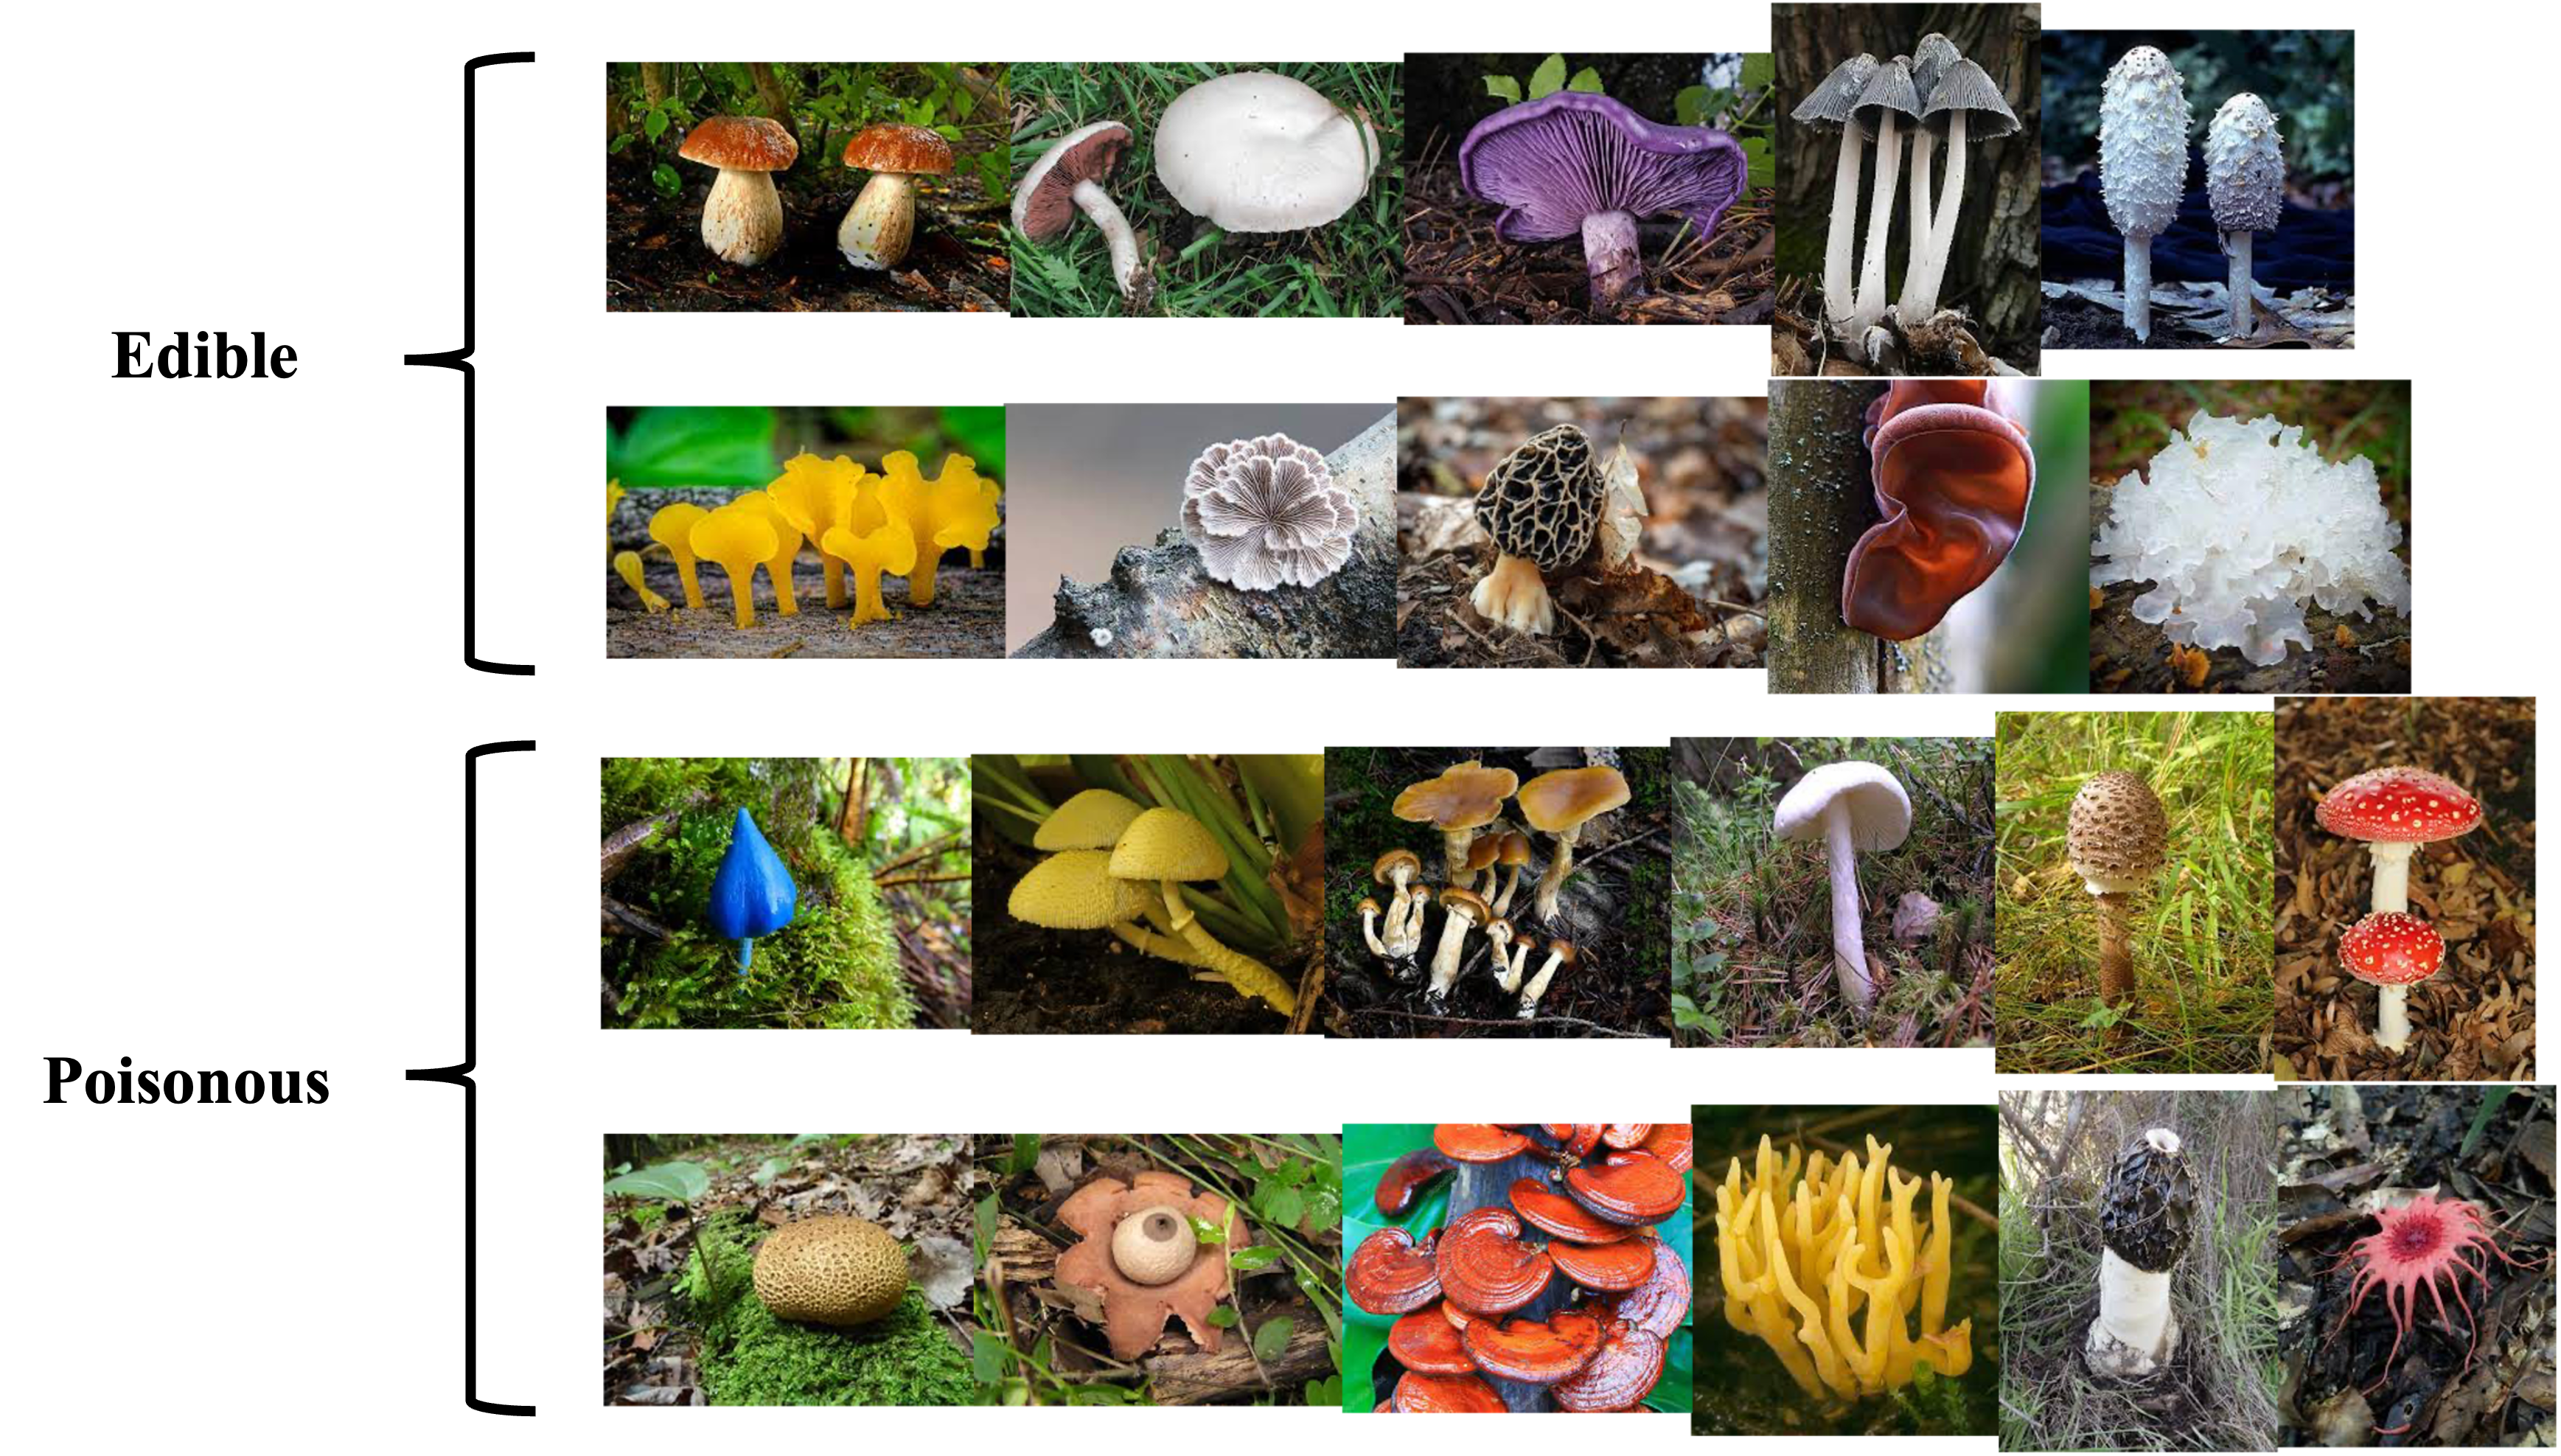
\includegraphics[width=5in]{STA221Template/Latex Template/Picture1.png}
\end{figure}

\end{appendices}

\end{document}

